\section{Data dependent task-optimized streams}
\label{sec:data_dep_streams}

In previous section we demonstrated that different tasks may need different streams. For example,
PSNR stream significantly underperforms the histogram stream when applied to the histogram
query~(\Cref{fig:histogram-comparison}).
Unfortunately, there is no single definition of best stream is for a given query. It could be a stream that
exhibit small changes in the data or stream that reaches the smallest error fastest.
Moreover, it is common to stop the streaming in case the quantity of interest is good enough or the data size
reached the limit of the machine.

We define the best stream as
a sequence of refinements that reach the minimum error at given stopping bit budget. Alas, in interactive application
we can only make assumptions what will be the number of bits streamed before user decides to stop the streaming. For
example, if a user drasticly changes viewpoint in a volume rendering application, the stream starts almost from scratch.
Taking the lack of control over the stopping budget to the extreme, the best stream becomes the one which minimizes
the error at all bit budgets. However, as in any optimization problem we may reach local minimum, as
chunks that improve the error but have impact on later refinement will have lower priority. The existence of local
minima prevents this progressive stream to be globally optimal.
We can compute the optimal stream by searching the ordering space for one that is optimal for the largest number
of bit budgets. Unfortunately, finding such ordering is exponential in number of chunks. Therefore, we focus on
finding a greedy scheme that could be good representative for the optimal stream. There are two primary directions
along which we can greedily search for sream: fine-to-coarse or coarse-to-fine.

\paragraph*{Fine-to-coarse greedy algorithm} utilizes full dataset to construct the stream.
Moreover,
if we wanted to precompute stream order which could be utilized during query, we would have access to whole
data set and could compute this stream. The algorithm is in principle a reverse of the previous approach, the
stream is constructed by starting with full data set and one by one disabling the chunks. At each step, a chunk
with smallest errorr impact is disabled (TODO: more detail). This algorithm is still of greedy nature as it
makes only locally optimal choice. Similarly to the coarse-to-fine algorithm, the running time is still $O(n^3)$.

\begin{figure}
        \centering
        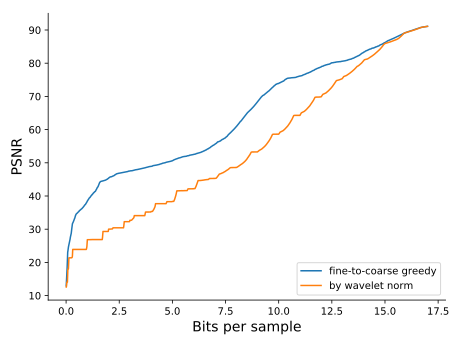
\includegraphics[width=0.48\linewidth]{img/figure4_new/rmse-miranda-viscosity}
        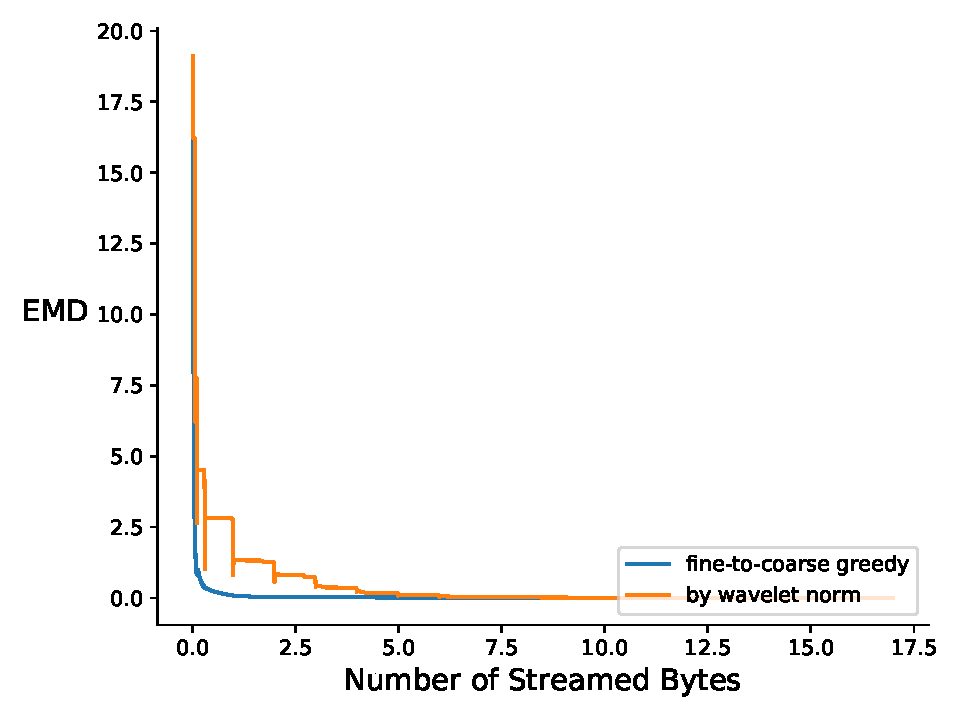
\includegraphics[width=0.48\linewidth]{img/figure4_new/histogram-miranda-viscosity}
        \caption{Comparison of fine-to-coarse and by wavelet norm (TODO: by wavelet norm is 4x4 blocks but the coarse-to-fine is 16x16 blocks due to slowness; I could recompute by wavelet norm with 16x16 blocks) streams on Miranda viscosity data set.
                 On the left is stream optimized for PSNR (higher is better) and on the right for histogram (lower is better).}
\end{figure}


\paragraph*{Coarse-to-fine greedy algorithm} starts with no data and the initial error is computed with respect
to the full data set. Then it takes a list of all chunks in the dataset, computes the error as if the chunk was
enabled, and picks the chunk with the highest absolute difference in the error with respect to the current error.
We use absolute difference to avoid the case where the error difference is zero or negative, which would result
in a long stream of chunk that do not decrease the error significantly. This assumption reflects the expectation
of more data meaning better result. The running time of this algorithm is $O(n^3)$ as we start with $n$ chunks
and at each streaming step decrease the chunk count by one. The cube factor comes from the need to perform inverse
wavelet transform and compute the error for each chunk.

Since the fine-to-coarse greedy stream outperforms the coarse-to-fine stream we further investigate possible
runtime optimizations. Surprisingly, only performing the first round of chunk error calculation and then sorting
those chunks by the error closely matches the full greedy algorithm. This simple optimization reduces the time
complexity to $O(n^2)$ and thus makes it more practical. We use this greedy scheme throught our evaluation named
\emph{fully adpative} stream.

\begin{figure}
        \centering
        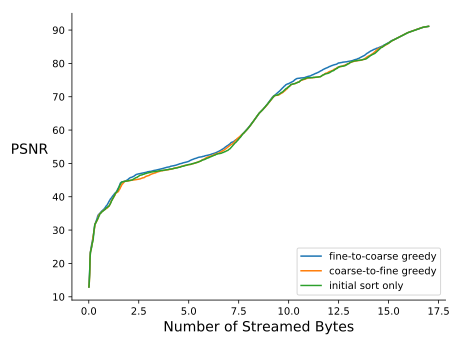
\includegraphics[width=0.48\linewidth]{img/figure6/rmse-miranda-viscosity}
        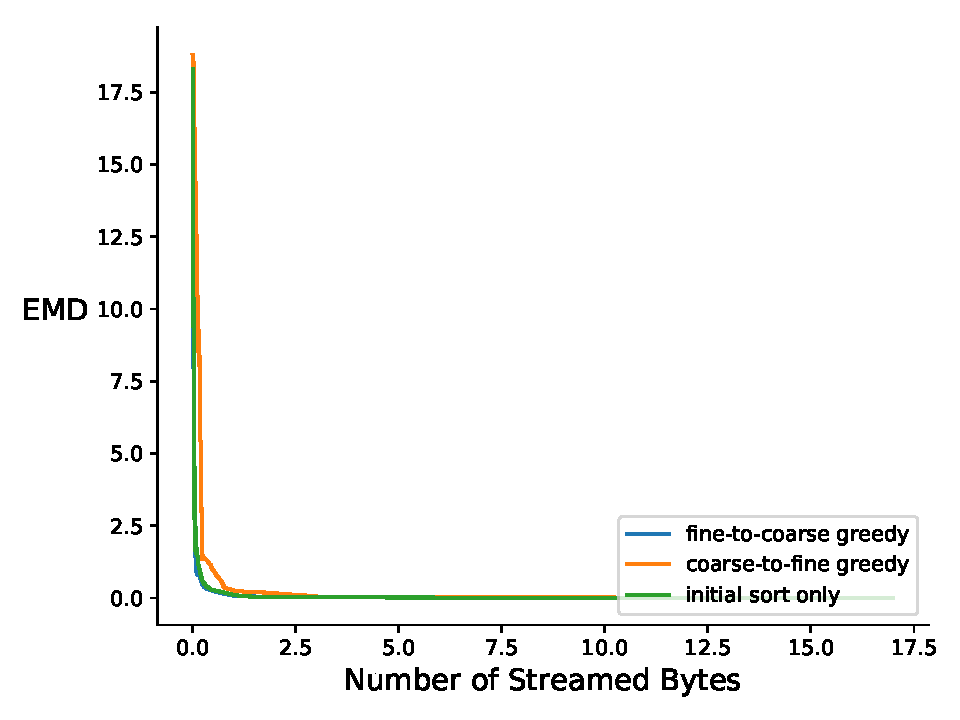
\includegraphics[width=0.48\linewidth]{img/figure6/histogram-miranda-viscosity}
        \caption{The fully adaptive stream (fine-to-coarse with only initial sorting) closely follows the coarse-to-fine and
                 fine-to-coarse streams both for PSNR and histogram.}
\end{figure}
